\documentclass[11pt,a4paper]{article}
\usepackage[margin=21mm]{geometry}
\usepackage[T1]{fontenc}
\usepackage{lmodern}
\usepackage{graphicx,booktabs,tabularx,amsmath,hyperref,float}
\hypersetup{colorlinks=true,linkcolor=blue,urlcolor=blue,
 pdftitle={Displaced/non-displaced EEG classification: feature, decoder and Graz-style comparisons},
 pdfauthor={Satyam Awasthi}}
\setlength{\parindent}{0pt}
\setlength{\parskip}{4pt}
\setlength{\emergencystretch}{2em}
\setlength{\tabcolsep}{5pt}
\newcommand{\uv}{\ensuremath{\mu\mathrm{V}}}
\title{Displaced/non-displaced EEG classification\\
\large Feature, decoder and Graz-style baseline comparisons}
\author{Satyam Awasthi}
\date{}
\begin{document}
\maketitle
\begin{abstract}
We evaluated single-trial decoding of displaced (D) versus non-displaced (ND) mouse-movement trials. An exploratory two-participant pilot compared four channel sets, three temporal representations and four preprocessing conditions. We then fixed three decoder configurations and evaluated them in 23 additional participants using identical no-FORCe trials and whole-recording holdouts, separately within each participant and session. Eight-channel shrinkage LDA with 100 ms mean-amplitude features achieved participant-weighted balanced accuracy of 76.3\% and ROC-AUC of 0.822, exceeding Cz/FCz LDA in 22/23 participants. A subsequent matched tree comparison gave 65.9\% balanced accuracy for these binned features versus 61.7\% for 100 training-fold-selected, Graz-style channel/time-point amplitudes. Results support the eight-channel LDA as a working personalised decoder. They do not establish cross-participant model transfer, an artifact-free signal or a specifically neural ErrP source.
\end{abstract}

\section{Questions and scope}
The preceding waveform audit identified useful class differences but could not establish which features would predict held-out trials. This note addresses four questions:
\begin{enumerate}
\setlength{\itemsep}{1pt}
\item Do 50 ms bins or individual samples improve on 100 ms means in the pilot?
\item Does the full montage add predictive information beyond the smaller scalp groups?
\item How do fixed shrinkage-LDA and decision-tree decoders compare on common data?
\item How do our binned features compare with a Graz-style top-100 amplitude representation under the same tree and validation scheme?
\end{enumerate}
\begin{table}[H]\centering\small
\begin{tabularx}{\linewidth}{@{}lXX@{}}\toprule
Analysis & Participants and trial selection & Processing scope\\\midrule
Exploratory LDA pilot & mle01 and spe30; 2,562 trials accepted in all four conditions & All four conditions; four channel sets and three temporal representations\\
Fixed decoder evaluation & 23 validation participants, with the two pilots separate; all accepted no-FORCe trials & BP no-FORCe only; fixed full LDA, central LDA and full tree\\
Graz-style feature follow-up & Same participants, eligible sessions and trial IDs as the fixed evaluation & BP no-FORCe only; six matched tree feature designs\\\bottomrule
\end{tabularx}
\caption{The four-condition processing comparison is pilot-only. The later full-dataset ranking concerns decoders under BP no-FORCe. The Graz-style feature comparison is a follow-up on the same validation cohort, not a new untouched test set.}\label{tab:scope}
\end{table}

\clearpage
\section{Data, preprocessing and inclusion}
\subsection{Participants and trial meaning}
The available data cover 25 participants and pre, post and retest sessions. mle01 and spe30 informed pilot feature and decoder choices. The remaining 23 participants evaluate those fixed choices; they are termed the validation cohort here. This is internal evaluation within the available study, not blinded external validation. Each personalised decoder is trained on other recordings from the same participant and session.

D denotes target-displaced trials; ND denotes non-displaced trials. These are task labels, not independent annotations of error awareness or of the neural source of a response. Movement onset is $t=0$. Recorded EEG has eight channels at 500 Hz: P3, PO3, PO7, CP5, CP1, Cz, FCz and FC1.

\subsection{No-FORCe reference and quality checks}
The full-dataset analysis reuses saved no-FORCe epochs with continuous, zero-phase, fourth-order Butterworth 1--20 Hz filtering. Final analysis epochs are $[-1,1)$ s, baseline-corrected by the channel mean over $[-0.2,0)$ s. A trial is rejected if any channel exceeds 100 \uv{} in absolute amplitude anywhere in that two-second epoch. No FORCe or other reconstructive cleaning is applied.

Raw loss codes, timestamp gaps and nonfinite EEG are checked across the complete $[-1.5,1.5)$ s context. Two-second guards exclude the edges of valid continuous segments. The three-second context is a quality gate for this reference; it is not a new segment-level filtering operation. Event validation precedes signal acceptance. Recordings with no validated events remain documented and are not rescued using classifier outcomes.

The saved reference signals and acceptance decisions were checked against all 29 pilot control recordings and matched exactly. The full analysis includes every trial passing the no-FORCe rules; it does not require acceptance by any FORCe condition.

\begin{table}[H]\centering\small\setlength{\tabcolsep}{3.4pt}
\begin{tabular}{@{}lrrrrrrr@{}}
\toprule
Cohort & $N$ & Event-valid & Accepted & Evaluated & ND & D & Sessions \\
\midrule
Validation & 23 & 32329 & 27666 & 27645 & 18378 & 9267 & 67 \\
Pilots & 2 & 2881 & 2565 & 2565 & 1681 & 884 & 6 \\
\bottomrule
\end{tabular}

\caption{Trial inclusion by cohort. $N$ is participants; Event-valid is before signal-quality exclusion; Accepted is after the no-FORCe quality rules; Evaluated additionally requires an evaluable recording-wise split. ND and D counts refer to evaluated trials. Sessions are participant/session combinations.}\label{tab:retention}
\end{table}
There are 380 inventoried recordings, 357 with validated events. Across both cohorts, 30,231 trials pass quality checks; 30,210 enter cross-validation. The validation cohort contributes 27,645 evaluated trials and 67 sessions; the pilots contribute 2,565 trials and six sessions.

\subsection{Evaluation eligibility and missing coverage}
A session must have at least two recordings with accepted trials and both classes in every training fold. rle13/pre has only one accepted recording (10 trials), while vco27/pre has two accepted recordings (11 trials) but a training fold with only one class. These sessions cannot support the fixed protocol. Their retention counts remain reported, and the other sessions from those participants remain eligible.

A single-class \emph{test} recording is still predicted. Its run AUC and run balanced accuracy are undefined; all its predictions still contribute to session-level confusion counts. Two of the 349 evaluated held-out recordings have this limitation. Their undefined AUCs are omitted from run-AUC averaging and the denominator is recorded.

\clearpage
\section{Features, decoders and validation}
\subsection{Binned and sample-level representations}
Each channel contributes seven consecutive 100 ms means (50 samples each) over $[0.2,0.9)$ s. Pilot alternatives are fourteen 50 ms means or all 350 original samples per channel over the same interval. Vectors retain separate channels.
\begin{table}[H]\centering\small
\begin{tabular}{@{}llrrr@{}}\toprule
Set & Channels & 100 ms & 50 ms & Samples\\\midrule
Central & Cz, FCz & 14 & 28 & 700\\
Centroparietal & CP1, CP5 & 14 & 28 & 700\\
Posterior & P3, PO3, PO7 & 21 & 42 & 1,050\\
Full & All eight & 56 & 112 & 2,800\\\bottomrule
\end{tabular}
\caption{Feature counts. Set names identify electrode groups, not isolated cortical sources. Full overlaps the other groups and also includes FC1.}\label{tab:features}
\end{table}

\subsection{Fixed decoder settings}
\textbf{Shrinkage LDA.} Training-fold feature scaling precedes LDA with automatic covariance shrinkage and equal priors. The scikit-learn 1.9.1 settings are \texttt{solver=lsqr}, \texttt{shrinkage=auto}, and priors $(0.5,0.5)$ \cite{sklda}. Neither scaling nor covariance estimation uses the held-out recording.

\textbf{Decision tree.} All tree comparisons use the same binary CART configuration: Gini impurity, best splits, all supplied features available at each split, unrestricted depth, minimum split size 2, minimum leaf size 1, no post-pruning and equal sample weights. The seed is 20261027. These are explicit fixed default assumptions, not settings recovered from the Graz implementation \cite{sktree}. No hyperparameter or decision-threshold search is performed.

The tree retains empirical training-class proportions, while LDA uses equal priors. Their comparison therefore concerns the configured decoders, including class handling, rather than model architecture alone. The unpruned tree can produce pure-leaf scores of 0 or 1; its within-run AUC can then equal its balanced accuracy. These probabilities are not calibrated.

\subsection{Whole-recording holdouts and metric definitions}
Within each participant/session, leave one entire recording run out and train on the others. All configurations share identical held-out trial IDs and labels. Every evaluated trial receives one out-of-fold prediction per configuration. There is no cross-session pooling or cross-participant training. The fixed full-dataset evaluation uses 349 folds per decoder (1,047 fits across three decoders).

D is the positive class. For session-level pooled held-out counts,
\[
\mathrm{Sensitivity}_D=\frac{TP}{TP+FN},\quad
\mathrm{Specificity}_{ND}=\frac{TN}{TN+FP},\quad
\mathrm{BA}=\frac{\mathrm{Sensitivity}_D+\mathrm{Specificity}_{ND}}{2}.
\]
Overall accuracy is also reported because it appears in the Graz analysis, but depends on class proportions. AUC is calculated within each two-class held-out run and then averaged, avoiding a primary AUC that mixes score scales from separately fitted models.

For cohort summaries, average the eligible sessions $S_i$ within each participant, then the $N$ participants equally. Trial counts do not determine participant weights:
\[
\overline M=\frac{1}{N}\sum_{i=1}^{N}\frac{1}{|S_i|}\sum_{s\in S_i} M_{is}.
\]


\clearpage
\section{Exploratory pilot: features and processing sensitivity}
\subsection{Channel sets and temporal resolution}
The pilot uses 2,562 common trial IDs from 29 recordings and six participant/session combinations. Selection is matched across all processing conditions. Pilot waveforms and scores informed later choices and remain exploratory.
\begin{table}[H]\centering
\begin{tabular}{@{}lrrr@{}}
\toprule
Channel set & 100 ms & 50 ms & Samples \\
\midrule
Central & 74.8 & 72.7 & 72.8 \\
Centroparietal & 71.1 & 70.7 & 69.6 \\
Posterior & 71.6 & 70.8 & 70.4 \\
Full & 80.7 & 79.7 & 78.7 \\
\bottomrule
\end{tabular}

\caption{Mean session balanced accuracy (\%) for primary BP no-FORCe in the matched pilot. Each participant contributes three sessions, so the six-session mean also weights the two participants equally. Samples retain 350 original time points per channel.}\label{tab:pilot_resolution}
\end{table}
Full with 100 ms means has the highest primary-condition mean BA (80.7\%) and exceeds Central in five of six sessions. Finer representations offer no consistent advantage. Strong descriptive separation at Cz/FCz therefore does not establish optimal multichannel decoding; additional channels can contribute joint information without identifying its physiological source.

The 56-feature Full representation was carried forward. Binning may conceal narrow waveform detail while retaining useful predictive information; these are different assessment criteria.

\subsection{Four-condition comparison is confined to the pilot}
Condition 1 applies continuous 1--20 Hz bandpass without FORCe. Condition 2 applies the same bandpass before three independent one-second FORCe calls. Condition 3 applies continuous 1 Hz high-pass and a 20 Hz low-pass on the three-second segment without FORCe. Condition 4 inserts the three one-second FORCe calls before that low-pass. All use three-second context and a two-second crop; cleaning joins are at $-0.5$ and $+0.5$ s. The feature interval includes the latter join. These are not the historical two-half epochs joined at movement onset.
\begin{table}[H]\centering\small\setlength{\tabcolsep}{3.6pt}
\begin{tabular}{@{}llrrrr@{}}
\toprule
ID & Processing & Central & Centroparietal & Posterior & Full \\
\midrule
1 & BP, no FORCe & 74.8 & 71.1 & 71.6 & 80.7 \\
2 & BP, FORCe & 68.5 & 66.1 & 66.5 & 78.3 \\
3 & Split, no FORCe & 74.6 & 71.2 & 71.3 & 80.9 \\
4 & Split, FORCe & 68.2 & 66.6 & 68.5 & 78.9 \\
\bottomrule
\end{tabular}

\caption{Matched pilot mean session BA (\%) with 100 ms features. Every entry uses the same 2,562 trials. Appendix~\ref{app:pilot} retains Full results separately by participant/session.}\label{tab:pilot_processing}
\end{table}
The two no-FORCe schemes are close in this descriptive summary; Full is 80.7\% for BP and 80.9\% for split filtering. FORCe changes prediction and is not uniformly favourable across individual sessions. Accuracy cannot establish artifact removal quality: contamination can itself predict task labels, and cleaning can change relevant and irrelevant signals.

BP no-FORCe was retained as the established working reference after the artifact-handling review, not selected as the largest entry in Table~\ref{tab:pilot_processing}. The full-dataset decoder and Graz-style comparisons below do \emph{not} rank all four preprocessing conditions across the dataset.

\clearpage
\section{Fixed configurations in the remaining participants}
\subsection{Participant-weighted primary results}
Table~\ref{tab:cohort} evaluates the fixed Full LDA, Central LDA and Full tree in the 23 participants outside the decoder-selection pilot. All three use 100 ms features over $[0.2,0.9)$ s, the same no-FORCe trials and the same whole-recording splits.
\begin{table}[H]\centering\small
\begin{tabular}{@{}lrrrrr@{}}
\toprule
Decoder & Acc. & BA & D recall & ND recall & AUC \\
\midrule
LDA, all eight & 77.0 & 76.3 & 74.4 & 78.2 & 0.822 \\
LDA, Cz/FCz & 70.8 & 70.3 & 69.0 & 71.7 & 0.756 \\
Tree, all eight & 69.2 & 65.9 & 56.1 & 75.7 & 0.659 \\
\bottomrule
\end{tabular}

\caption{Validation cohort: 23 participants, 67 eligible sessions and 27,645 evaluated trials. Acc., BA and both recalls are percentages; AUC is on $[0,1]$. Values first average eligible sessions within each participant, then participants equally.}\label{tab:cohort}
\end{table}
Full LDA reaches 76.3\% BA and AUC 0.822, with 74.4\% displaced recall and 78.2\% non-displaced recall. Central LDA reaches 70.3\% BA and AUC 0.756. The Full tree reaches 65.9\% BA and AUC 0.659, with a larger recall imbalance (56.1\% D versus 75.7\% ND).

Full LDA has higher participant-mean BA than Central in 22/23 participants. The mean paired advantage is 5.96 percentage points, calculated from unrounded values. cna07 is the small reversal (84.8\% Full versus 85.0\% Central, rounded). Full LDA participant means range from 56.8\% to 87.4\%; the cohort mean does not imply uniform individual performance.

These results support the additional montage information in this personalised decoding setup. They do not localise it to the posterior electrodes: Full also adds FC1, and the comparison includes different feature counts and covariance structures. The tree comparison concerns an untuned, unpruned baseline; it is not evidence that every possible tree configuration is inferior to LDA.

\subsection{What is and is not validated}
The fixed cohort evaluation assesses whether a configuration chosen in two participants remains useful in the other available participants, while training each decoder on that participant's own data. It does not measure transfer of an already trained model to another participant or session. Prior exploratory work on this dataset also means the cohort is not a blinded external test.

Results are descriptive; no population significance test or confidence interval is claimed. No participant or session was removed because of a poor classification score. The two exclusions follow the prespecified ability to form training/test folds. Participant summaries use the remaining eligible sessions, with those coverage differences explicit in the figures and appendix.

The later Graz-style designs were examined after these fixed results. Their use of the same cohort is a follow-up comparison, not independent confirmation of a newly selected feature pipeline.

\clearpage
\subsection{Participant-level consistency}
\begin{figure}[H]\centering
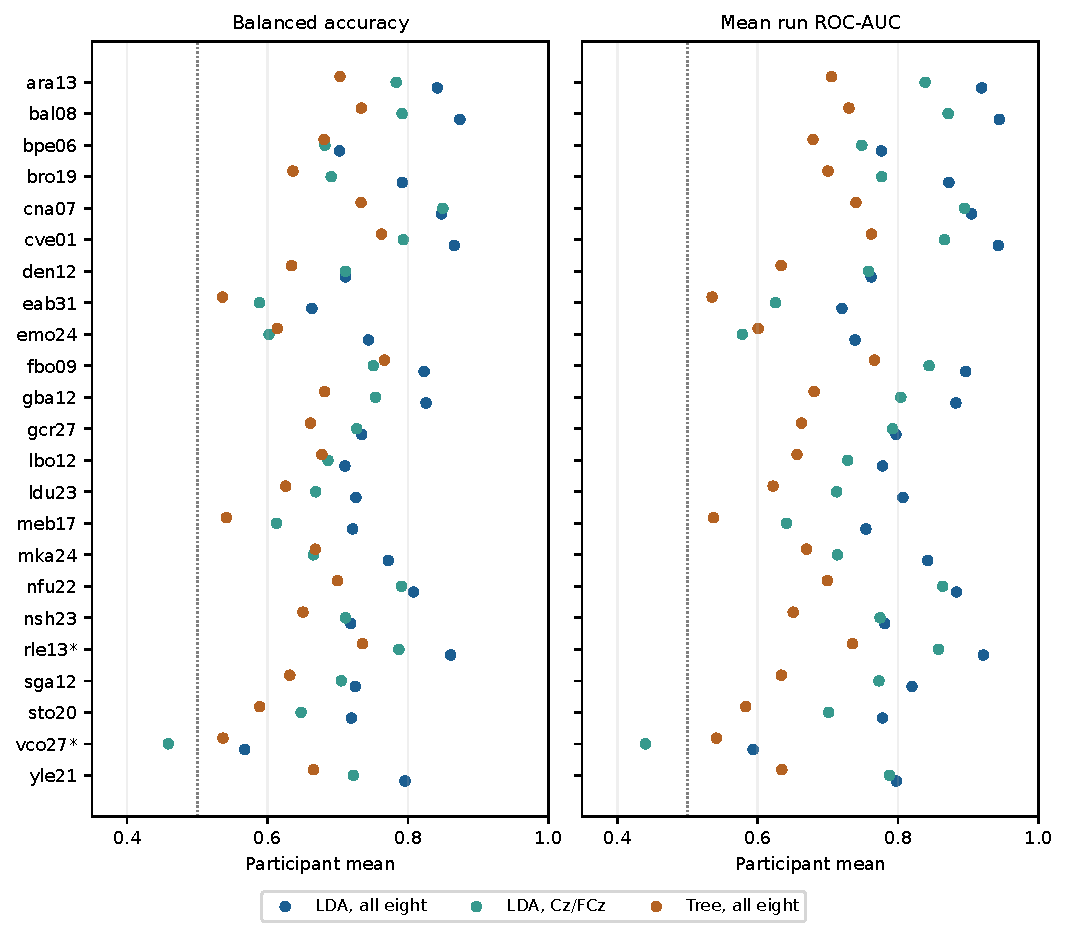
\includegraphics[width=\linewidth]{figures/participant_scores.pdf}
\caption{Each point is one validation participant's mean across eligible sessions. Left: pooled out-of-fold BA within sessions, then session and participant aggregation. Right: run AUCs averaged within sessions, then sessions. The same accepted trials and held-out recordings underlie all three decoders. Asterisks mark rle13 and vco27, whose pre sessions are not evaluable; all others contribute three sessions. The dotted line is the 0.5 reference, not a significance threshold.}\label{fig:participants}
\end{figure}
Full LDA generally improves both BA and AUC, but differences vary. The participant and session displays should accompany the mean rather than presenting 76.3\% as a common performance level. Appendix~\ref{app:participants} provides numerical participant results, and Appendix~\ref{app:sessions} retains the separate session view.

\clearpage
\section{Graz-style amplitude selection and matched tree features}
\subsection{Published specification and explicit interpretation}
The Graz paper reports a binary decision tree, 10-fold cross-validation and 100 channel/time-point amplitude features ranked by training-fold $r^2$ \cite{graz}. It describes $[-1,+1]$ s epochs but does not separately specify a narrower classification candidate interval. In particular, it does not report a $[0.2,0.9)$ s restriction; that interval is our feature-design choice.

We therefore evaluate two raw-amplitude pools: all 8,000 channel/time pairs from the documented two-second epoch $[-1,1)$ s, and the 2,800 pairs from $[0.2,0.9)$ s. Full-epoch selection is an explicit interpretation of the reported epoch, not an independently recovered implementation detail. The response-interval control lets us compare feature methods over a common interval. A selected amplitude is one channel at one time; the 100 selected pairs need not represent 100 distinct clock times.

For training-fold feature $f_j$ and binary label $y$, rank by
\[
r_j^2=\frac{\left[\sum_{i\in\mathcal T}(f_{ij}-\bar f_{j,\mathcal T})(y_i-\bar y_{\mathcal T})\right]^2}
{\left[\sum_{i\in\mathcal T}(f_{ij}-\bar f_{j,\mathcal T})^2\right]
 \left[\sum_{i\in\mathcal T}(y_i-\bar y_{\mathcal T})^2\right]}.
\]
$\mathcal T$ contains training trials only. Recompute the top 100 in every fold, with fixed channel/time order for ties and zero for constant-feature scores. This matches the squared-Pearson definition in the shared legacy ranking helper. No held-out sample or label participates in ranking.

\subsection{Six tree feature designs on the same data}
Both raw models and the four binned channel-set trees share the same tree settings, no-FORCe trial IDs and existing holdouts. The four binned designs use seven 100 ms means per channel over $[0.2,0.9)$ s. The Full-bin predictions are reused exactly from Table~\ref{tab:cohort}; the five other designs are new fits.
\begin{table}[H]\centering\small\setlength{\tabcolsep}{3.5pt}
\begin{tabular}{@{}lrrrrrr@{}}
\toprule
Feature design & $p$ & Acc. & BA & D recall & ND recall & AUC \\
\midrule
Top 100 $r^2$, $[-1,1)$ s & 100 & 65.3 & 61.7 & 50.5 & 72.8 & 0.618 \\
Top 100 $r^2$, $[0.2,0.9)$ s & 100 & 64.9 & 61.2 & 49.8 & 72.6 & 0.614 \\
100 ms, Central & 14 & 67.7 & 64.4 & 54.4 & 74.4 & 0.645 \\
100 ms, Centroparietal & 14 & 67.0 & 63.6 & 53.2 & 73.9 & 0.636 \\
100 ms, Posterior & 21 & 67.1 & 63.6 & 53.3 & 73.9 & 0.636 \\
100 ms, Full & 56 & 69.2 & 65.9 & 56.1 & 75.7 & 0.659 \\
\bottomrule
\end{tabular}

\caption{Participant-weighted validation results for the six matched trees ($N=23$, 67 sessions). $p$ is inputs to the tree; percentage columns are Acc., BA, D recall and ND recall. AUC is unscaled. Raw selection has 8,000 or 2,800 candidate amplitudes before retaining 100.}\label{tab:graz}
\end{table}
Full-epoch top-100 amplitudes achieve 61.7\% BA; restricting candidates to the response interval gives 61.2\%. These similar means do not establish interval equivalence. Full-bin features achieve 65.9\%, an advantage of 4.27 percentage points over full-epoch selection under this matched tree protocol. The smaller binned groups achieve 63.6--64.4\%. This compares feature designs including their different dimensionalities, not temporal averaging alone.

\clearpage
\begin{figure}[H]\centering
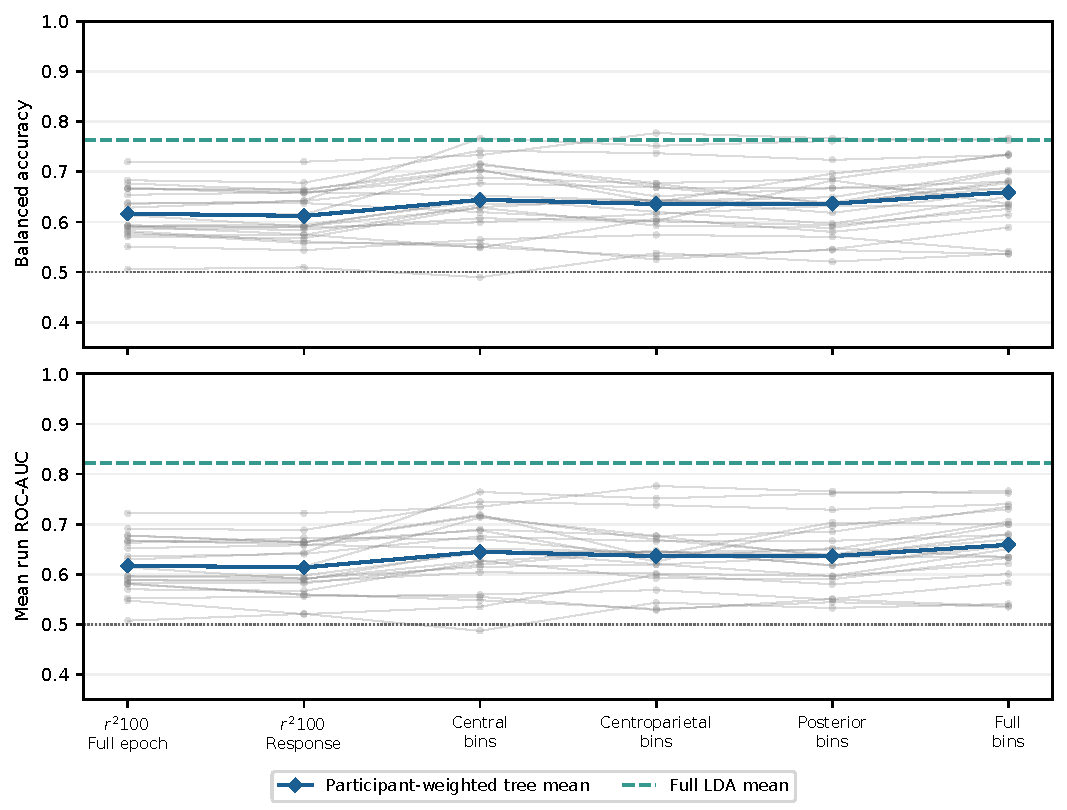
\includegraphics[width=\linewidth]{figures/graz_comparison.pdf}
\caption{Decision-tree feature comparison in the validation cohort. Thin grey lines link the same participant's eligible-session means; the blue line is the equal-participant mean. The first two designs use 100 training-selected raw amplitudes. The last four use 100 ms bin means over $[0.2,0.9)$ s. The dashed reference is the existing Full LDA mean on the same trials, with different class handling as described above. Lines are descriptive and are not confidence intervals.}\label{fig:graz}
\end{figure}
\subsection{Comparison to the paper and interpretation limits}
This provides a Graz-style feature-selection baseline with our data and evaluation protocol. It is not a reproduction of published performance: we retain no-FORCe preprocessing, a fourth-order filter, session-specific whole-recording holdouts and participant weighting. The paper describes FORCe, a third-order filter and 10-fold CV. Its detailed tree hyperparameters are not reported. Consequently, subtracting its published score from ours would not isolate a feature improvement.

The same-interval raw control strengthens the comparison of feature designs, but 100 selected amplitudes and 14--56 bin means still differ in dimensionality and redundancy. Selected raw samples may be adjacent, and a full-epoch pool can select pre-onset samples. Their occurrence is not evidence of a component latency or neural source. Selection frequencies across overlapping training folds are not independent observations.

All 698 top-100 selections were checked against an independent class-mean/variance form of squared Pearson correlation; the largest numerical difference was $1.44\times10^{-15}$. All 181,260 tree predictions and the exact shared trial IDs were verified. This checks implementation and bookkeeping, not physiological validity.

\section{Working conclusion}
Among the configurations evaluated across the 23 validation participants, \textbf{eight-channel shrinkage LDA with 100 ms mean amplitudes over $[0.2,0.9)$ s is the strongest working decoder}: 76.3\% BA, AUC 0.822. Its montage advantage persists beyond the two pilots. Our Full-bin feature design also scores higher than the Graz-style raw-amplitude design under the same fixed tree protocol.

This conclusion is conditional on the existing no-FORCe reference and personalised whole-run evaluation. It does not select the best preprocessing condition across the full dataset, identify a specifically neural ErrP, or establish that accepted trials are artifact-free. No further optimisation is undertaken here.

\begin{thebibliography}{9}
\raggedright
\bibitem{graz} I. Amaunam, M. Sultana, B. Rodriguez-Herreros, T. Tadi, R. Leeb and S. Perdikis.
\emph{EEG correlates of error-related activity during ballistic computer mouse movements}.
9th Graz Brain-Computer Interface Conference, 2024.
\url{https://repository.essex.ac.uk/38379/1/tDCS_ErrP_9th_Graz_BCI_Conference_2024.pdf}
\bibitem{sklda} scikit-learn. \emph{LinearDiscriminantAnalysis}, version 1.9.1 documentation.
\url{https://scikit-learn.org/stable/modules/generated/sklearn.discriminant_analysis.LinearDiscriminantAnalysis.html}
\bibitem{sktree} scikit-learn. \emph{DecisionTreeClassifier}, version 1.9.1 documentation.
\url{https://scikit-learn.org/stable/modules/generated/sklearn.tree.DecisionTreeClassifier.html}
\end{thebibliography}

\clearpage
\appendix
\section{Validation participant results}\label{app:participants}
\begin{table}[H]\centering\small\setlength{\tabcolsep}{4pt}
\begin{tabular}{@{}lrrrrrrr@{}}
\toprule
Participant & Sessions & Trials & LDA8 & LDA2 & Tree8 & $r^2$ full & $r^2$ resp. \\
\midrule
ara13 & 3 & 1325 & 84.2 & 78.3 & 70.3 & 66.8 & 66.0 \\
bal08 & 3 & 1261 & 87.4 & 79.2 & 73.4 & 66.6 & 66.5 \\
bpe06 & 3 & 1140 & 70.3 & 68.2 & 68.1 & 63.6 & 64.2 \\
bro19 & 3 & 816 & 79.2 & 69.1 & 63.6 & 63.8 & 63.8 \\
cna07 & 3 & 994 & 84.8 & 85.0 & 73.3 & 68.3 & 67.8 \\
cve01 & 3 & 1405 & 86.6 & 79.3 & 76.2 & 72.0 & 72.0 \\
den12 & 3 & 1364 & 71.1 & 71.1 & 63.4 & 61.4 & 59.1 \\
eab31 & 3 & 1423 & 66.3 & 58.9 & 53.6 & 58.2 & 56.1 \\
emo24 & 3 & 884 & 74.4 & 60.2 & 61.4 & 59.1 & 57.5 \\
fbo09 & 3 & 1332 & 82.3 & 75.1 & 76.7 & 62.8 & 64.2 \\
gba12 & 3 & 1414 & 82.6 & 75.4 & 68.1 & 65.4 & 65.9 \\
gcr27 & 3 & 1439 & 73.4 & 72.7 & 66.1 & 57.1 & 56.8 \\
lbo12 & 3 & 1265 & 71.0 & 68.6 & 67.7 & 57.4 & 57.4 \\
ldu23 & 3 & 1275 & 72.6 & 66.9 & 62.6 & 58.6 & 58.5 \\
meb17 & 3 & 1010 & 72.1 & 61.3 & 54.1 & 55.1 & 54.4 \\
mka24 & 3 & 1398 & 77.2 & 66.5 & 66.8 & 59.3 & 59.4 \\
nfu22 & 3 & 1435 & 80.8 & 79.1 & 70.0 & 67.7 & 66.3 \\
nsh23 & 3 & 1442 & 71.8 & 71.1 & 65.0 & 59.0 & 59.0 \\
rle13 & 2 & 887 & 86.1 & 78.7 & 73.5 & 61.5 & 61.5 \\
sga12 & 3 & 1121 & 72.5 & 70.5 & 63.2 & 59.3 & 58.9 \\
sto20 & 3 & 1291 & 71.9 & 64.8 & 58.9 & 57.9 & 55.8 \\
vco27 & 2 & 612 & 56.8 & 45.9 & 53.7 & 50.5 & 50.9 \\
yle21 & 3 & 1112 & 79.6 & 72.2 & 66.5 & 66.7 & 65.7 \\
\bottomrule
\end{tabular}

\caption{Participant mean BA (\%) across eligible sessions. LDA8 and LDA2 use 100 ms means from all eight channels and Cz/FCz, respectively. Tree8 uses all-channel 100 ms means. The last two columns are the top-100 raw-amplitude trees from the full epoch and response interval. Trials count unique evaluated trials, shared by every decoder. No participant is weighted by that count in cohort means.}\label{tab:participants}
\end{table}
Only the pre sessions of rle13 and vco27 are excluded. Their post and retest sessions remain included, giving two eligible sessions for each. The small reversal for cna07 concerns BA; it does not change the groupwise conclusion that the Full montage usually adds useful information under this evaluation.

\clearpage
\section{Separate session view}\label{app:sessions}
\begin{figure}[H]\centering
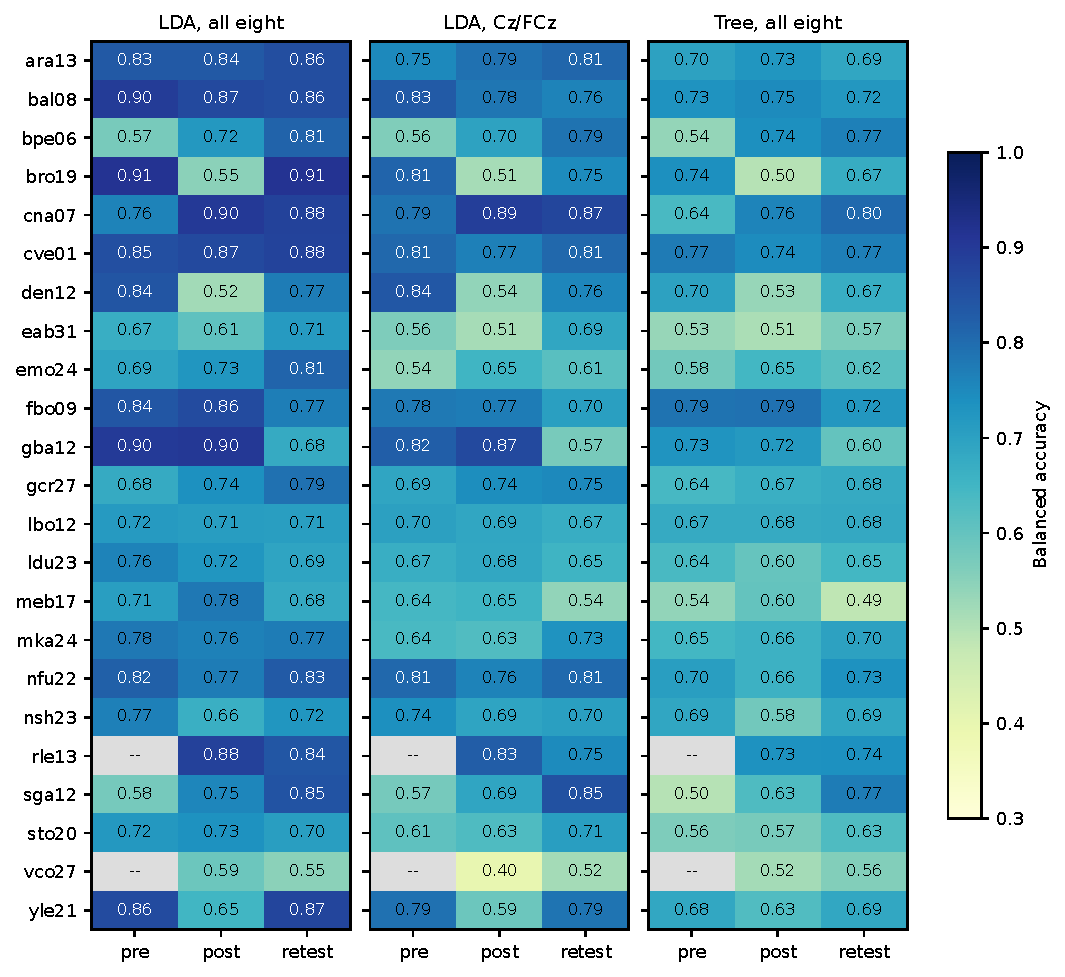
\includegraphics[width=\linewidth]{figures/session_scores.pdf}
\caption{Validation session BA for the three fixed decoders, with common colour scale and common trial selection. Grey cells are the two sessions that cannot support the recording-wise protocol. Performance changes across pre, post and retest differ by participant; the pooled cohort ranking does not imply a uniform session effect.}\label{fig:sessions}
\end{figure}

\clearpage
\section{Pilot processing results and acceptance-set distinction}\label{app:pilot}
\begin{table}[H]\centering\small\setlength{\tabcolsep}{4pt}
\begin{tabular}{@{}llrrrr@{}}
\toprule
Participant & Session & Condition 1 & Condition 2 & Condition 3 & Condition 4 \\
\midrule
mle01 & pre & 66.7 & 68.0 & 67.0 & 70.5 \\
mle01 & post & 73.8 & 70.0 & 74.2 & 71.4 \\
mle01 & retest & 86.7 & 83.6 & 86.7 & 82.9 \\
spe30 & pre & 89.8 & 87.0 & 90.3 & 86.3 \\
spe30 & post & 94.3 & 89.5 & 94.3 & 89.2 \\
spe30 & retest & 73.1 & 71.6 & 73.1 & 72.9 \\
\bottomrule
\end{tabular}

\caption{Full-montage 100 ms LDA BA (\%) for each matched pilot session. Conditions are defined in Table~\ref{tab:pilot_processing}. All use the same 2,562 trial IDs, so changes here do not arise from different accepted trial sets.}\label{tab:pilot_sessions}
\end{table}
For example, FORCe with split filtering improves this pilot score for mle01/pre but reduces it for other sessions. Such variability and the two-participant sample limit claims about preprocessing superiority. Classification is not an artifact-removal benchmark.

\begin{table}[H]\centering\small
\begin{tabular}{@{}lrrrrr@{}}
\toprule
Decoder & Acc. & BA & D recall & ND recall & AUC \\
\midrule
LDA, all eight & 80.4 & 80.8 & 82.2 & 79.5 & 0.859 \\
LDA, Cz/FCz & 74.7 & 74.7 & 74.5 & 74.8 & 0.797 \\
Tree, all eight & 73.2 & 70.0 & 59.7 & 80.3 & 0.701 \\
\bottomrule
\end{tabular}

\caption{The two pilots refitted under the later \emph{all-accepted no-FORCe} protocol: 2,565 trials, six sessions. Percentages except AUC. These rows accompany the fixed validation results but are not counted among the 23 validation participants.}\label{tab:pilot_refit}
\end{table}
The three additional trials relative to the matched pilot come from removing the requirement for acceptance in all four processing conditions. Training sets therefore also change. For example, Full LDA is 80.8\% in these refits versus 80.7\% in the original matched BP pilot; the small difference is not a new method effect. Earlier outputs are preserved.

The original Central-only tree experiment is likewise distinct from the later Full-montage tree. The tree feature follow-up evaluates the same 2,565 accepted pilot trials separately; its pilot scores are not used as independent confirmation of either feature design.
\end{document}
